\chapter{Resultados y Discusión}
\label{resultadosdiscusion}
\ifpdf
  \graphicspath{{Chapter6/Chapter6Figs/PNG/}{Chapter6/Chapter6Figs/PDF/}{Chapter6/Chapter6Figs/}}
\else
  \graphicspath{{Chapter6/Chapter6Figs/EPS/}{Chapter6/Chapter6Figs/}}
\fi

\markboth{\hfill \thechapter. Resultados y Discusión}{\hfill \thechapter. Resultados y Discusión}

\section{Ambiente de Ejecución.}

Las pruebas para la obtención de los resultados se ejecutaron en una computadora personal con la siguiente configuración:
\begin{itemize}
   \item Procesador Intel\textcopyright{}  Core\texttrademark{} i5 2.3 GHz.
    \item Memoria RAM de 8 GB. 
    \item Disco SSD de 256 GB.
    \item Sistema Operativo Linux Mint en su version 18.3 Cinnamon 64-bit.
\end{itemize}

% Para la puesta en marcha de la aplicación \textit{TapeYty} lo requerimientos no funcionales son los siguientes:

% \begin{enumerate}
%     \item 
% \end{enumerate}

\section{Resultados Obtenidos.}

En esta sección se presenta un análisis de los resultados obtenidos con \textit{TapeYty}.
La ``Fig.~\ref{fig:RecorridoActualZona83}'' muestra el camino trazado por el GPS instalado en el vehículo recolector 129 en la zona 83 de trabajo. Se puede observar que varios segmentos de calles son atravesados repetidas veces. La distancia total recorrida fue de 16.940 km. En la práctica, los recolectores suelen acumular las bolsas de basura de varias casas en una esquina, evitando que el conductor entrase a ciertas calles. Lastimosamente no se puede asegurar que dichos segmentos hayan recibido el servicio. Las avenidas de color naranja, que delimitan la zona, no forman parte de la recolección, pero de igual manera algunos segmentos de estas avenidas fueron utilizadas para poder acceder a las calles que si deben ser cubiertas por el servicio.

Por otra parte, en la ``Fig.~\ref{fig:RecorridoTapeYtyZona83}'' se muestra el camino generado por \textit{TapeYty}, tiene una cobertura total de las calles que deben ser visitadas en la zona. La secuencia se encuentra especificada en los segmentos. La metodología de trabajo se mantiene de acuerdo con lo establecido por la DSU como en la ``Fig.~\ref{fig:RecorridoActualZona83}'', y por lo tanto, la misma delimitación de zonas.

Las calles sin salida, las estrechas y las que limitan una zona pero que no deben ser visitadas necesariamente son gestionadas mediante \textit{TapeYty}. En el módulo de rutas de la aplicación el usuario tiene la posibilidad de modificar propiedades de las calles como ser el sentido, si se encuentra inhabilitada, o si es opcional el paso del camión por un segmento de calle determinado. Por ejemplo, en la ``Fig.~\ref{fig:RecorridoTapeYtyZona83Opcionales}'' ciertos segmentos de calles pasan a ser opcionales para el paso de camiones simulando el procedimiento llevado a cabo por el equipo de recolección (``Fig.~\ref{fig:RecorridoActualZona83}'').

% Algunos recorridos generados por la aplicación pueden contener segmentos de calles que no pertenezcan a la zona seleccionada debido a que los segmentos de sentido único en los límites de zonas requiere de un buffer para incluir calles aledanhas produce un resultado infactible.
Algunas zonas tienen varios segmentos de calles de un único sentido, y si solo se utilizan los segmentos dentro de la zona, el resultado podría resultar infactible computacionalmente o más costoso en distancia, por ello se agrega una banda perimetral, tal como en \citet{Braier2017AnArgentina}, de 220 metros representada como arcos auxiliares. Esta situación es común en la práctica actual de la recolección de residuos.

% \begin{figure}
%   \centering
%   \subcaption{Ruta actual.}{
%     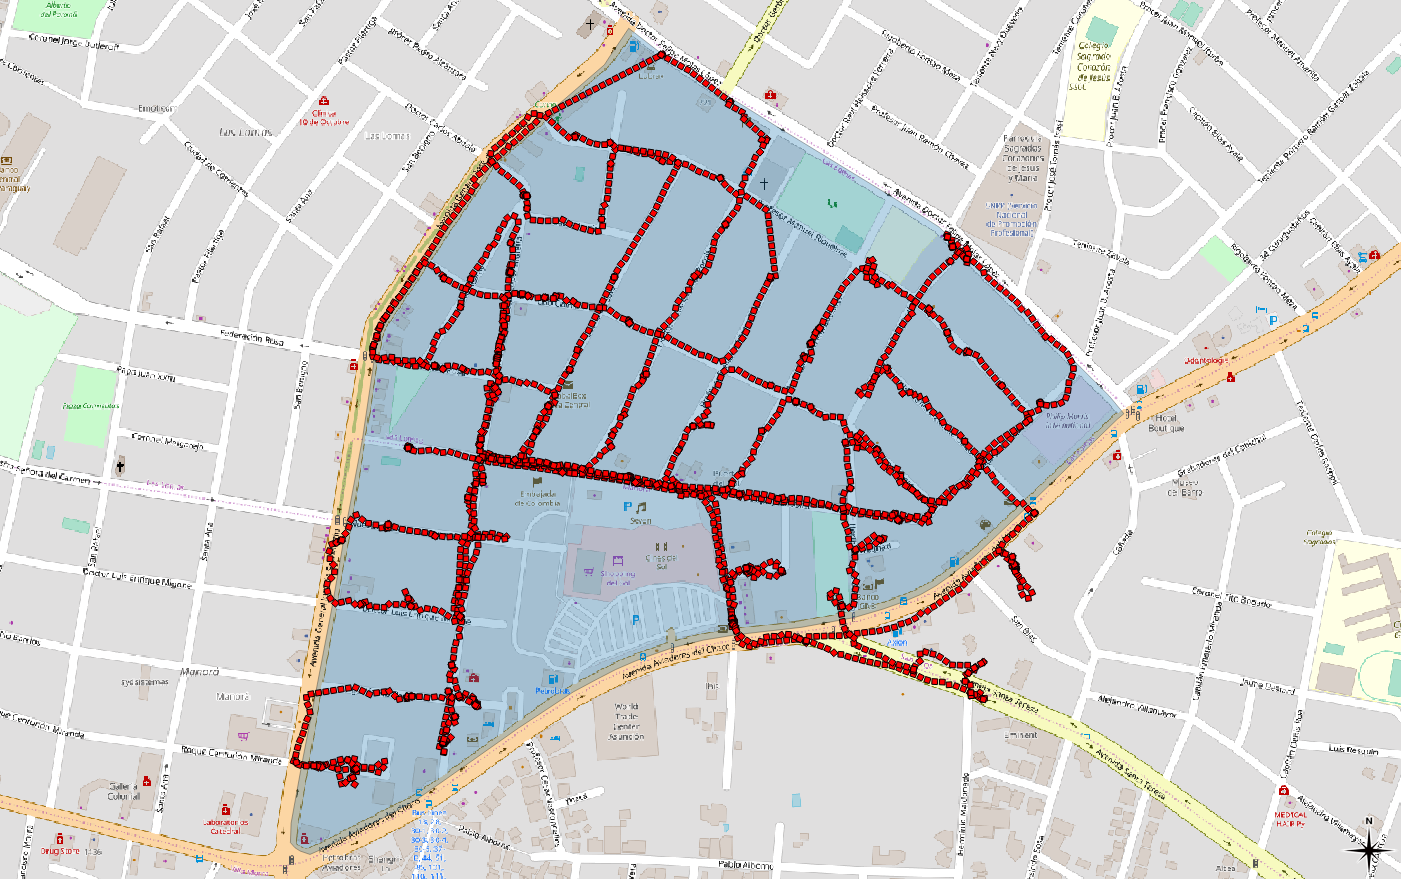
\includegraphics[width=0.45\textwidth]{recorrido83Actual.png}
%     \label{fig:RecorridoActualZona83}}%
%   \hfill
%   \subcaption{Ruta generada por \textit{TapeYty} con cobertura completa.}{
%     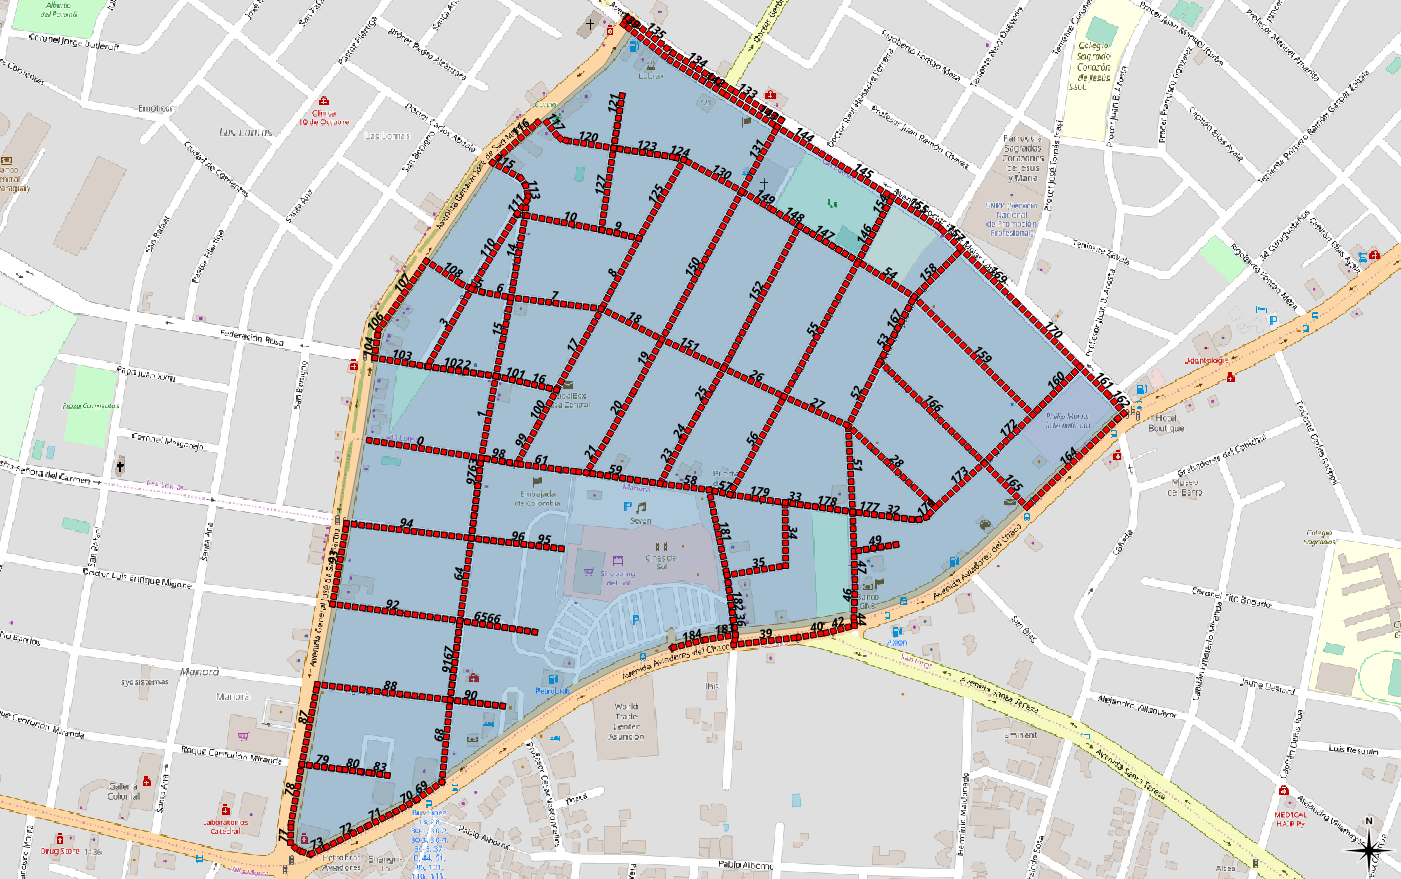
\includegraphics[width=0.45\textwidth]{recorrido83.png}
%     \label{fig:RecorridoTapeYtyZona83}}%
%   \hfill
%   \subcaption{Ruta generada por \textit{TapeYty} con segmentos opcionales.}{
%     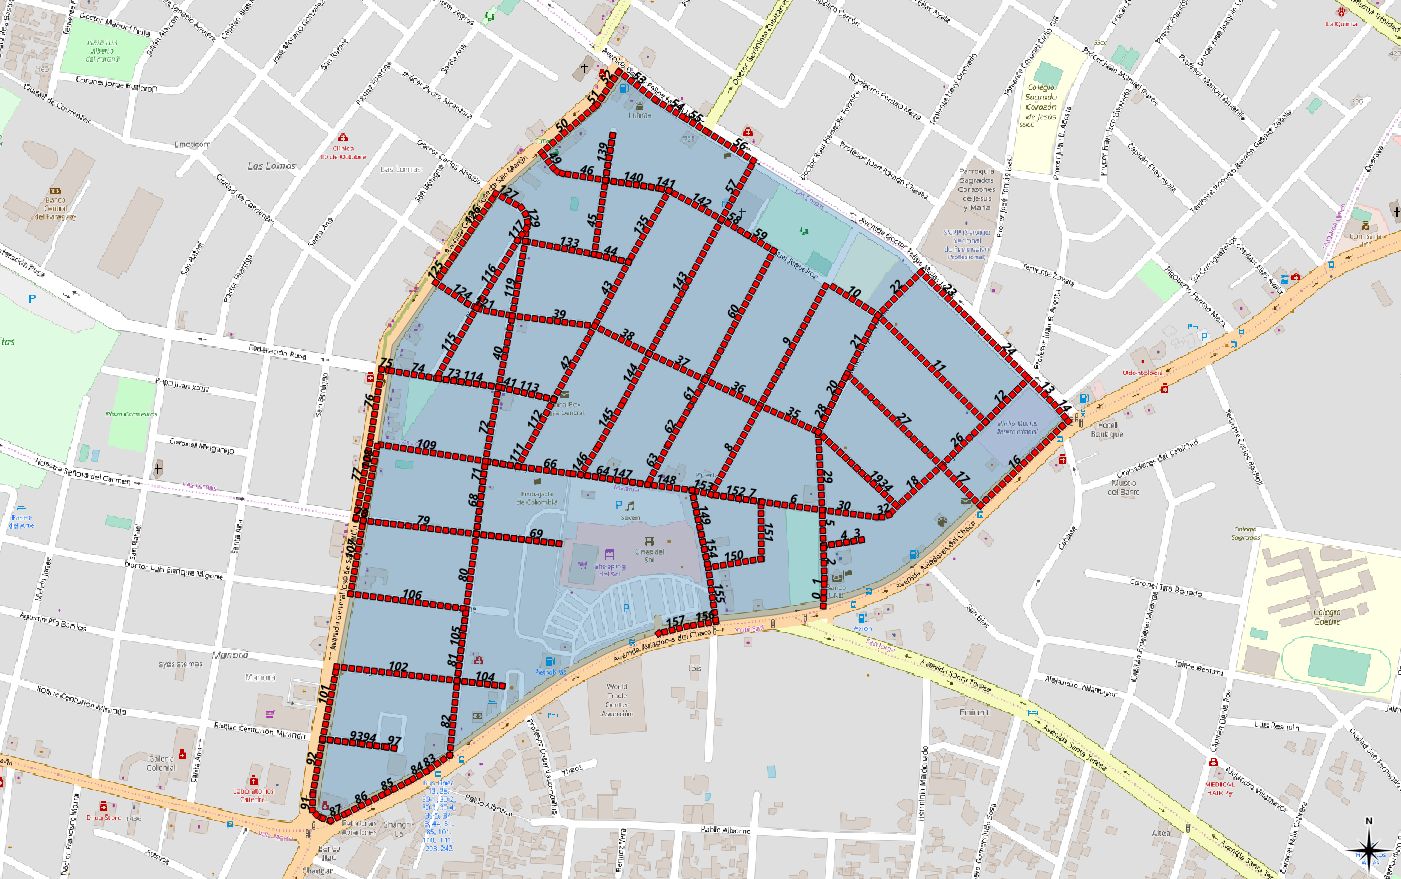
\includegraphics[width=1\textwidth]{recorrido83GeneradoNoHabilitados.png}
%     \label{fig:RecorridoTapeYtyZona83Opcionales}}%
%   \caption{Recorridos de la zona 83.}
% \end{figure}

% \begin{figure}[!ht]
%      \subfloat[First sub-figure]{
%       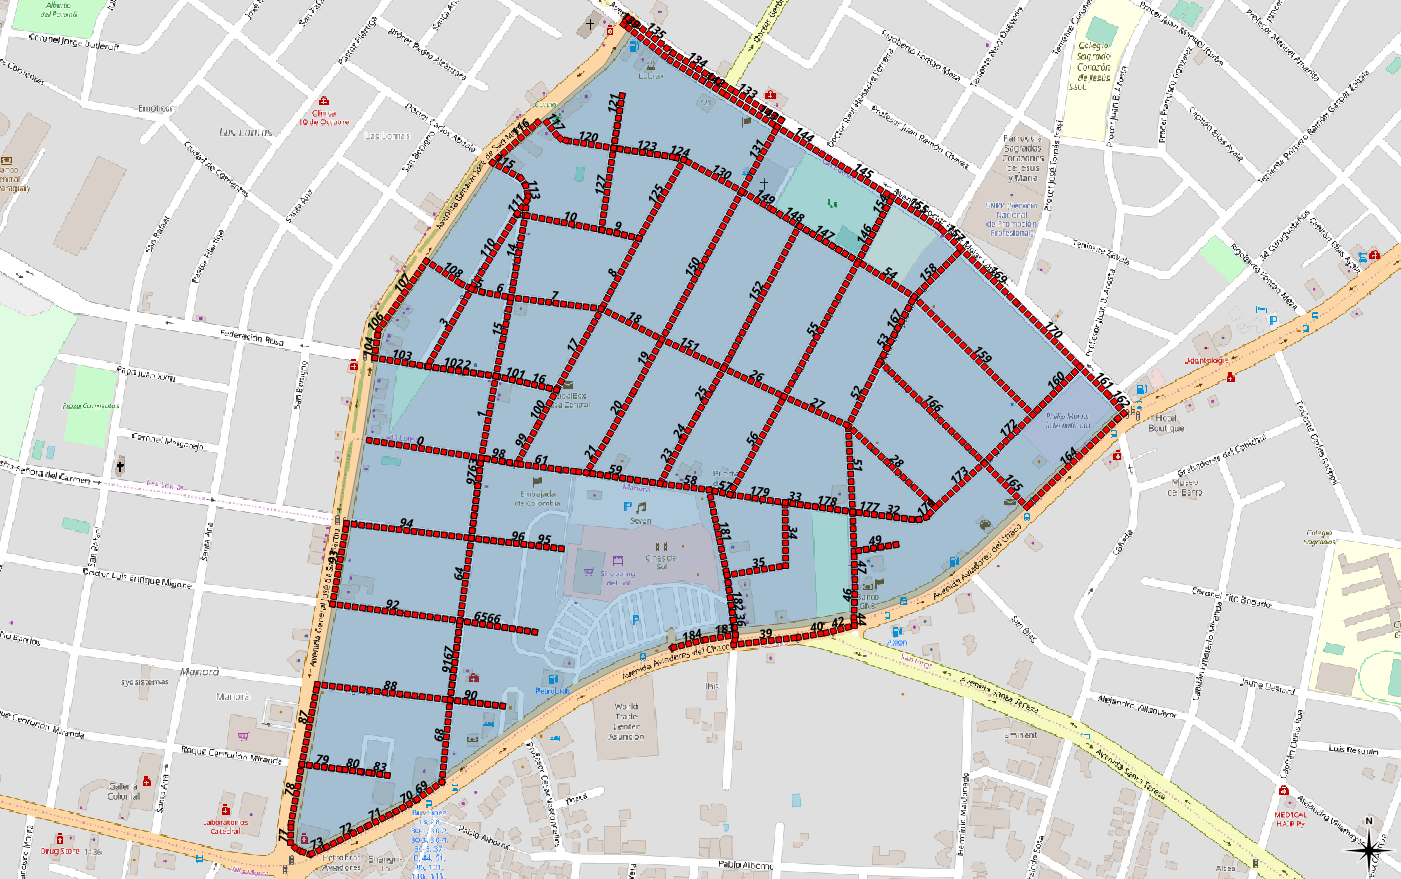
\includegraphics[width=0.45\textwidth]{recorrido83.png}
%       \label{subfig-1:dummy}
%      }
%      \hfill
%      \subfloat[First sub-figure]{
%       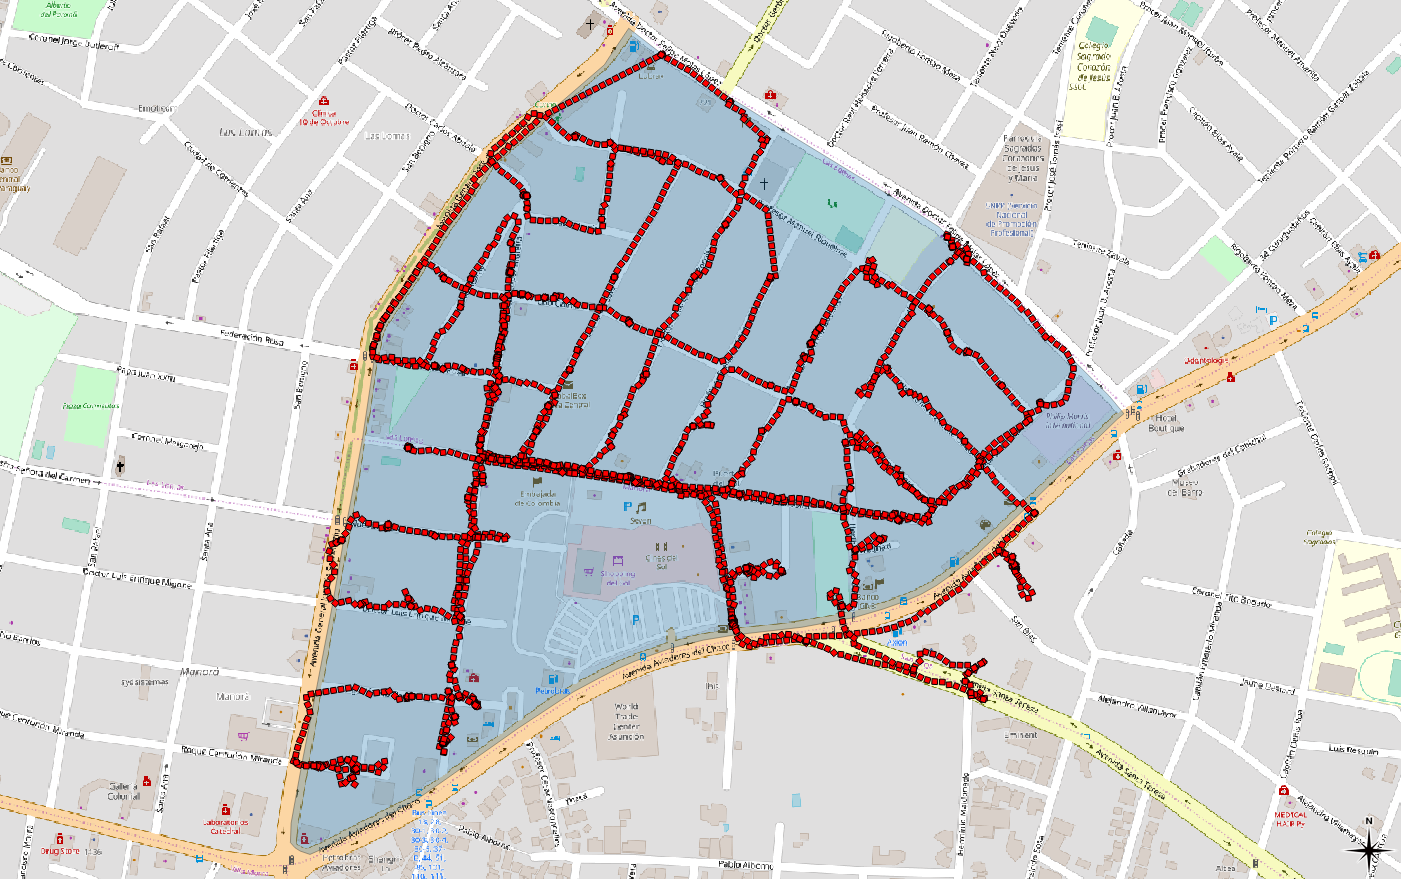
\includegraphics[width=0.45\textwidth]{recorrido83Actual.png}
%       \label{subfig-2:dummy}
%      }
%      \caption{Dummy figure}
%      \label{fig:dummy}
% \end{figure}

% \begin{figure}
%   \subfloat[]{%
%   \begin{minipage}{\linewidth}
%   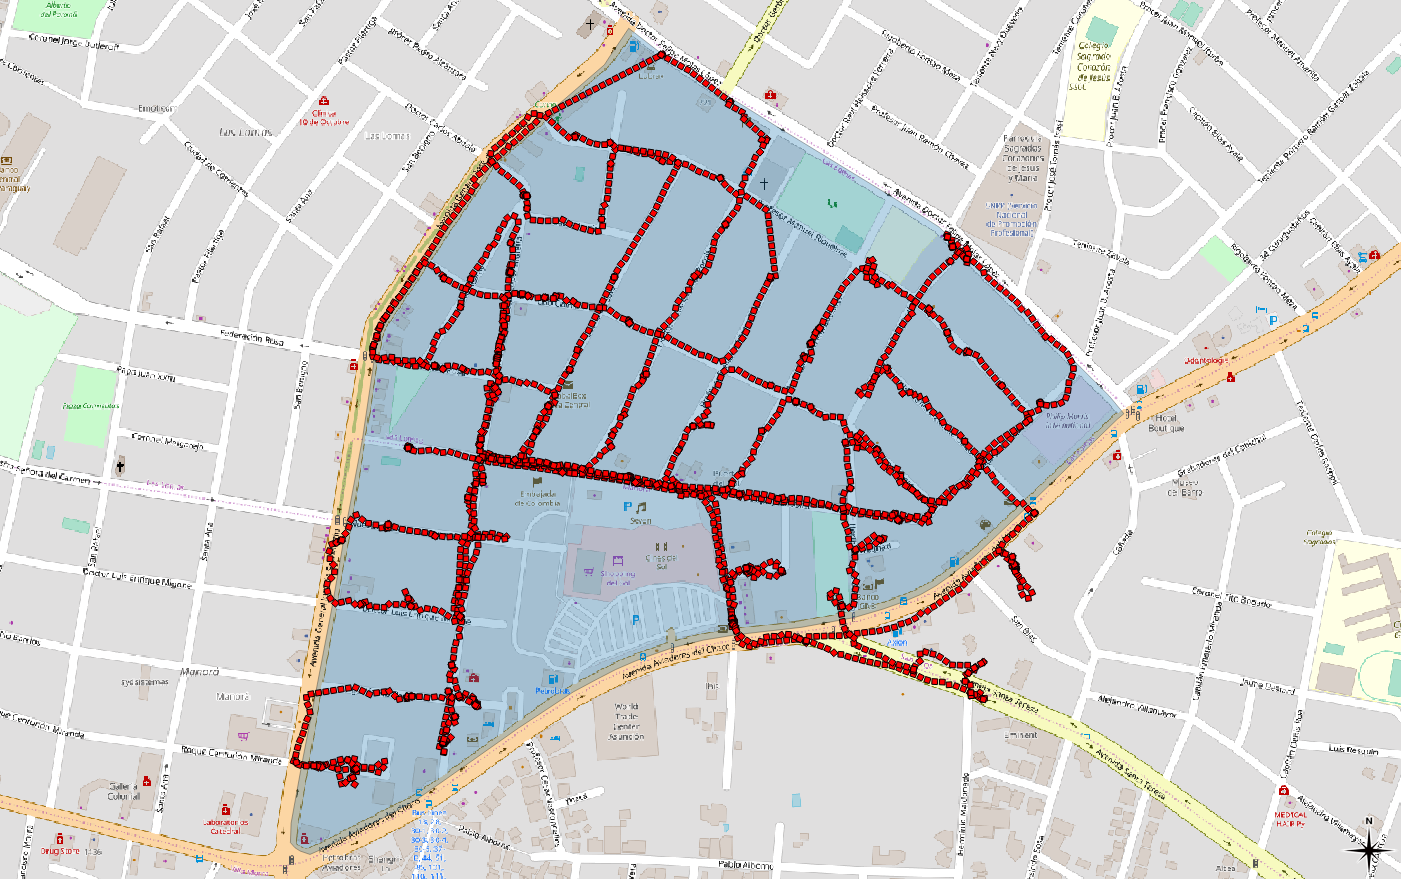
\includegraphics[width=.3\linewidth]{recorrido83Actual.png}\hfill
%   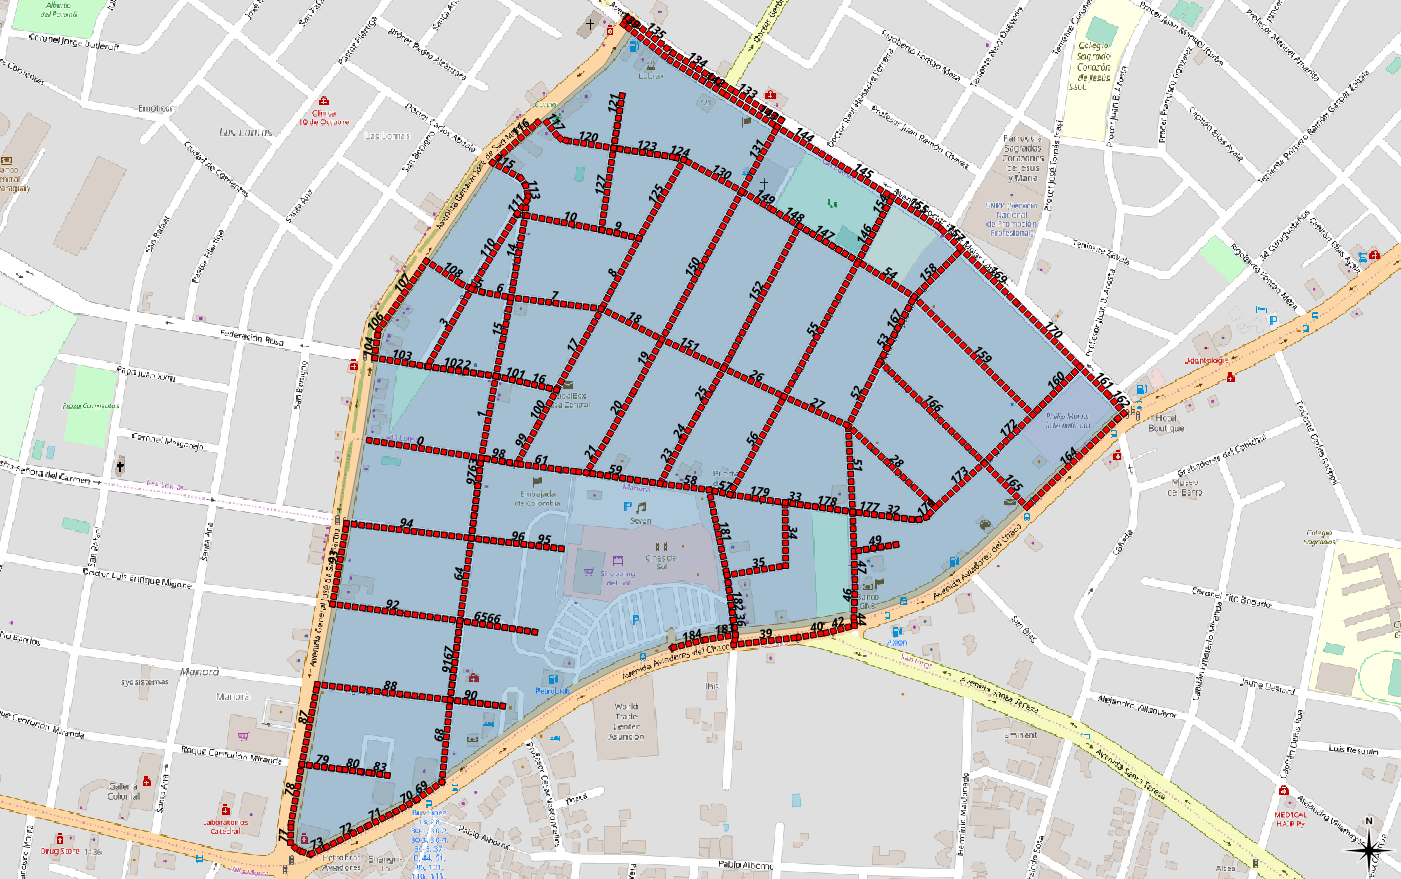
\includegraphics[width=.3\linewidth]{recorrido83.png}\hfill
%   \includegraphics[width=.3\linewidth]{example-image-a}%
%   \end{minipage}%
%   }\par
%   \subfloat[]{%
%   \begin{minipage}{\linewidth}
%   \includegraphics[width=.3\linewidth]{example-image-b}\hfill
%   \includegraphics[width=.3\linewidth]{example-image-b}\hfill
%   \includegraphics[width=.3\linewidth]{example-image-b}%
%   \end{minipage}%
%   }\par
%   \subfloat[]{%
%   \begin{minipage}{\linewidth}
%   \includegraphics[width=.3\linewidth]{example-image-c}\hfill
%   \includegraphics[width=.3\linewidth]{example-image-c}\hfill
%   \includegraphics[width=.3\linewidth]{example-image-c}%
%   \end{minipage}%
%   }
%   \caption{Some grouped images}
% \end{figure}

% \begin{figure*}[htbp]
%   \centering
%   \begin{subfig}[b]{0.45\textwidth}
%     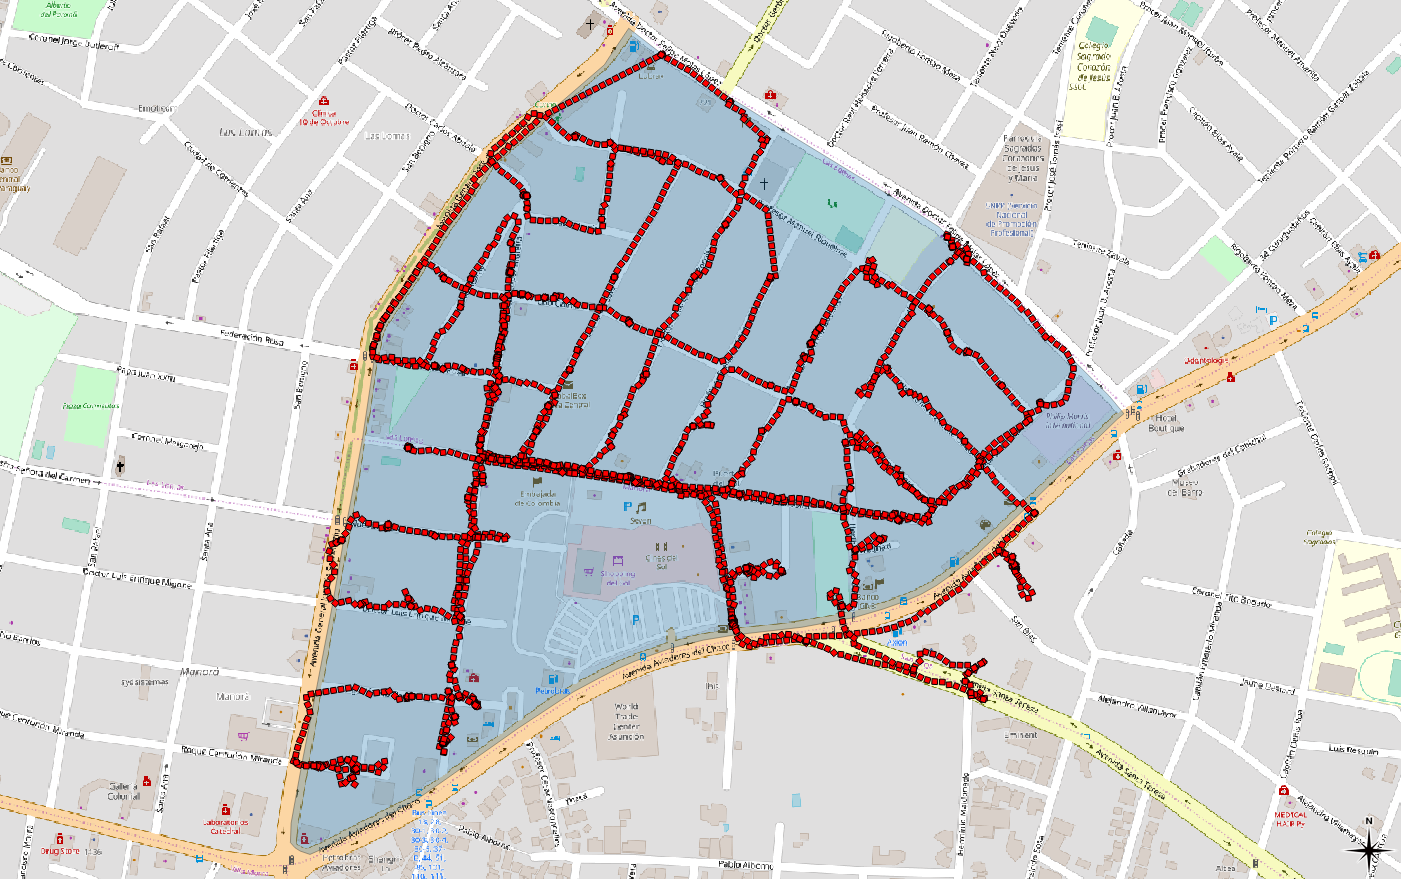
\includegraphics[width=\textwidth]{recorrido83Actual.png}
%     \caption{Ruta actual.}
%     \label{fig:RecorridoActualZona83}
%   \end{subfig}
%   \hfill
%   \begin{subfig}[b]{0.45\textwidth}
%     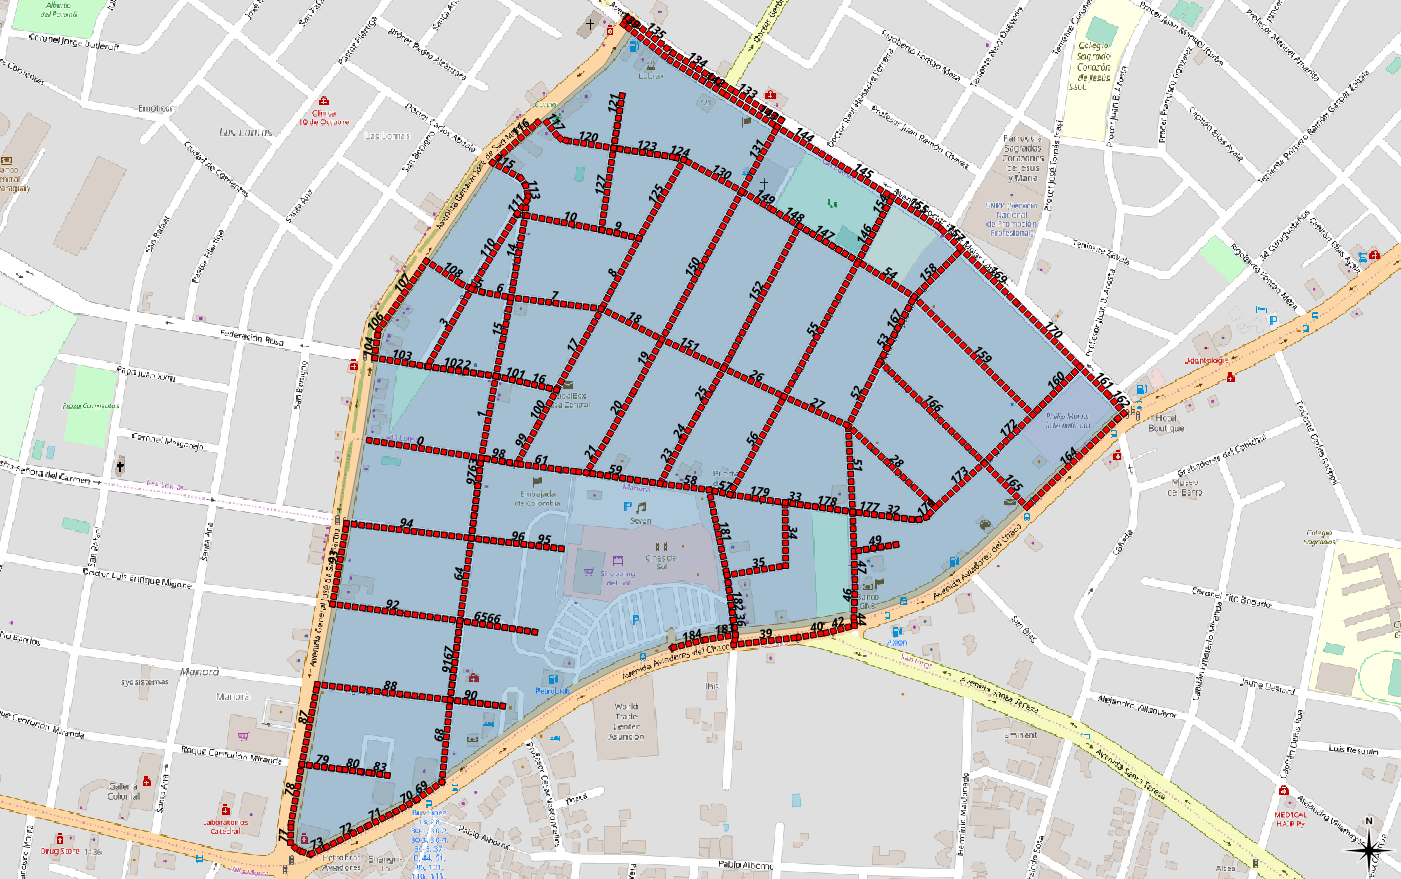
\includegraphics[width=\textwidth]{recorrido83.png}
%     \caption{Ruta generada por \textit{TapeYty} con cobertura completa.}
%     \label{fig:RecorridoTapeYtyZona83}
%   \end{subfig}
%   \begin{subfig}[b]{1\textwidth}
%         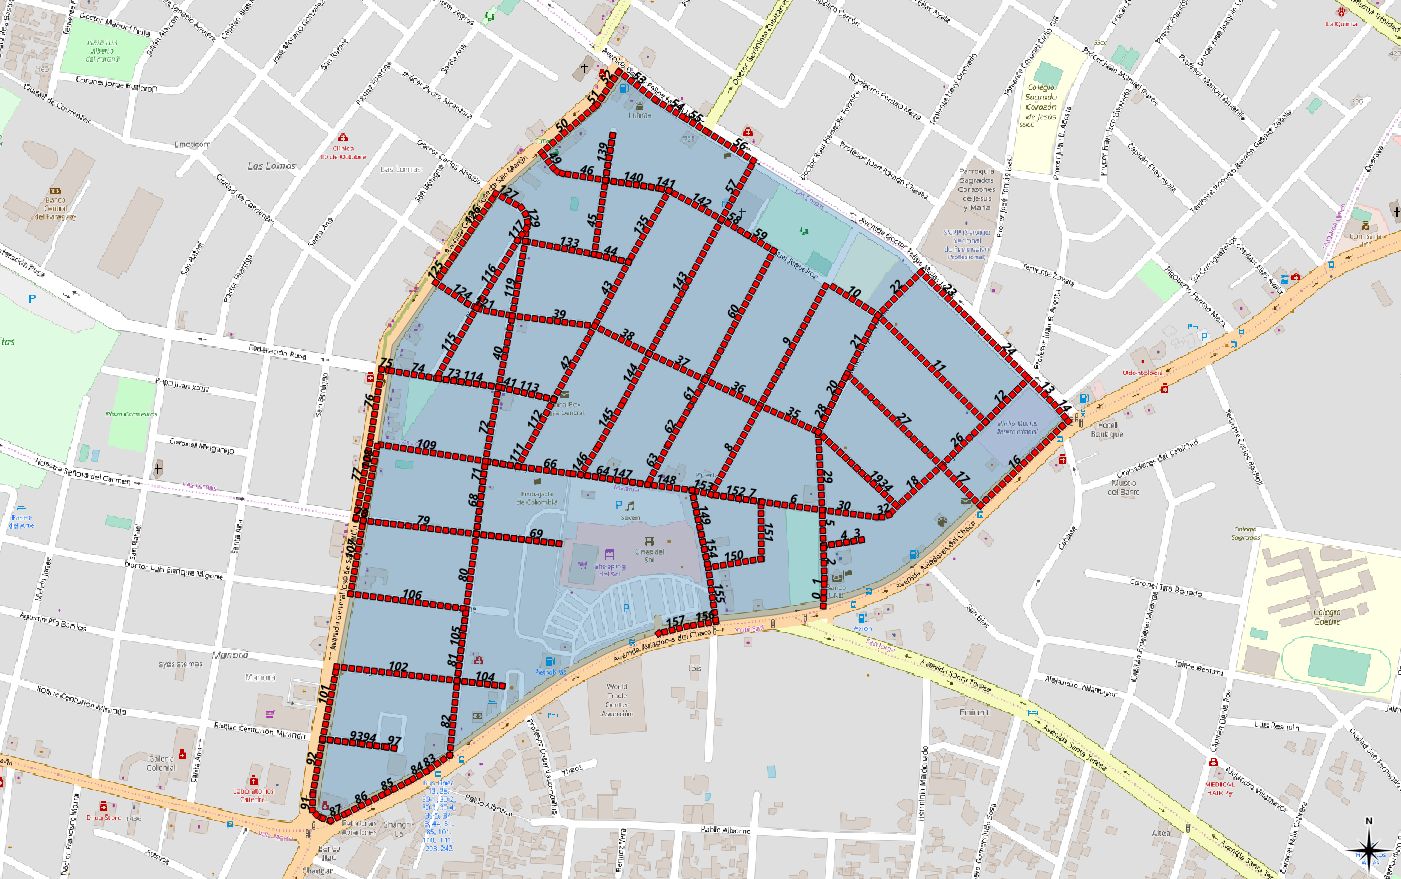
\includegraphics[width=\textwidth]{recorrido83GeneradoNoHabilitados.png}
%         \caption{Ruta generada por \textit{TapeYty} con segmentos opcionales.}
%         \label{fig:RecorridoTapeYtyZona83Opcionales}
%     \end{subfig}
%   \caption{Recorridos de la zona 83.}
% \end{figure*}

En el cuadro \ref{table:comparacionZona83} se presenta el análisis realizado sobre la zona 83.  En la primera columna se detallan las características de la zona, la segunda columna se refiere al escenario en el que todos los segmentos de calles deben ser visitados por el vehículo recolector y en la tercera columna se refiere al escenario en el que 5 segmentos de calles de sentido único y 3 de doble sentido fueron marcados como opcionales desde la aplicación. Ambos escenarios coinciden en la cantidad de vértices en el grafo, cantidad de calles de sentido único y de doble sentido, no así en la cantidad de arcos auxiliares, debido a la cantidad de segmentos opcionales. 

En el primer escenario es posible resolver mediante la técnica de mezcla de subtours recién en la tercera iteración, mientras que en el segundo se puede resolver con la misma técnica ya en la primera iteración, por ello se observa que el tiempo de ejecución del modelo es levemente menor para el segundo escenario. Realizar la expansión del grafo a partir de los datos de entrada es el paso que requirió de mayor tiempo en la aplicación. En ambos escenarios se redujo la distancia con respecto al recorrido actual, en el primero en un 20.31\%  y en el segundo un 26.31\%, con 3.44105 km. y 4.45612 km. menos respectivamente.

\begin{table}[htbp]
\caption{Resultados y análisis para la zona 83}
\begin{tabular}{lll}
\hline
\multirow{2}{*}{Zona 83}                            & \multicolumn{2}{l}{Cobertura de segmentos de calles} \\ \cline{2-3} 
                                                    & Sin opcionales           & Con opcionales           \\ \hline
$|V|$                                                   & 1352                     & 1352                     \\
$|E|$                                                   & 420                      & 420                      \\
$|AM|$                                                  & 256                      & 256                      \\
$|Aaux|$                                                & 1567                     & 1578                     \\
Iteraciones                                         & 3                        & 1                        \\
Tiempo de expansión (s)                      & 21.20426                 & 20.27737                 \\ 
Tiempo de ejecución de modelo (s)            & 0.73509                  & 0.22427                  \\ 
Tiempo de secuenciación (s)                  & 0.07936                  & 0.06370                  \\ 
Distancia (km)                                      & 13.49895                 & 12.48388                 \\ 
Mejor con respecto al actual (\%) & 20.31                    & 26.31                    \\ \hline
\end{tabular}
\label{table:comparacionZona83}
\end{table}
